\documentclass[9pt,conference]{IEEEtran}
\usepackage[nomarkers]{endfloat}
\usepackage[cmex10]{amsmath}
\usepackage{filecontents}
\usepackage{lipsum}
\usepackage{graphicx}

\begin{filecontents*}{informe.bib}
@electronic{refmallba,
  author        = {Michael Shell},
  title         = {{IEEE}tran Homepage},
  url           = {http://neo.lcc.uma.es/mallba/easy-mallba/index.html},
  year          = {2008}
}
\end{filecontents*}

\begin{document}

%-------- Metadata -------- 
	\title{Pr\'actico 1}
	\markboth{Algoritmos Evolutivos 2015}{Shell \MakeLowercase{\textit{et al.}}: A Novel Tin Can Link}
	\author{
		\IEEEauthorblockN{Gonzalo Torterolo}
		\IEEEauthorblockA{
			Facultad de ingenier\'ia\\
			UDELAR\\
			Montevideo, Uruguay\\
			Email: gonzalo.torterolo@fing.edu.uy
		}
		\and
		\IEEEauthorblockN{Gisel Cincunegui}
		\IEEEauthorblockA{
			Facultad de ingenier\'ia\\
			UDELAR\\
			Montevideo, Uruguay\\
			Email: gisel.cincunegui@fing.edu.uy
		}
	}



% ------- Contenido -------
	\maketitle

	\begin{abstract}
	En el presente informe el objetivo es probar las ventajas y limitaciones de las actuales librerias que implementan algoritmos gen\'eticos mediante la resoluci\'on de 2 problemas t\'ipicos de computaci\'on. Adem\'as se realizan pequeños analisis de las soluciones con el fin de verter conocimientos te\'oricos adquiridos en el curso.
	\end{abstract}
	\begin{IEEEkeywords}
	Algoritmos Evolutivos, AE, Algoritmos Gen\'eticos, AG, Malva, Mallba, Whatchmaker, Knapshak, Mochila
	\end{IEEEkeywords}

	\section{Introducci\'on}
	See \cite{refmallba} for more info

	En la consigna presentada (ver letra en \cite{refmallba}) se deben resolver dos variantes del problema de la mochila (explicadas en la consigna tambi\'en) utilizando ideas de los algoritmos gen\'eticos.

	Por otra parte, el an\'alisis y modelado del problema as\'i como las ventajas de utilizar este tipo de algorimos para el escenario queda relegado a una segunda instancia, pues ya estaban resueltos en las consignas. En todo momento prim\'o la aplicaci\'on de los conceptos te\'oricos del curso antes que la obtenci\'on de resultados como rendimiento, modularidad, etc. No nos interesa, por lo tanto, seguir aqu\'i un enfoque pr\'actico para esta primer aproximaci\'on a los algoritmos evolutivos donde ambos problemas son t\'ipicos y ampliamente estudiados.


	\subsection{Aplicaci\'on de AG}

	Se analizan las diferentes soluciones a las dos variantes del problema de la mochila aqu\'i presentadas, concluyendo con una implementaci\'on para ambos casos.
	Para comenzar a definir las soluciones a los problemas se debe determinar las siguientes car\'acter\'izticas de importancia para un AE t\'ipico.

	\begin{enumerate}
		\item Codificaci\'on.
		\begin{itemize}
				\item Tratamiento de codificaciones no factibles.
		\end{itemize}
		\item Poblaci\'on inicial.
		\begin{itemize}
				\item  Evaluaci\'on de coste/beneficio de utilizar criterios inteligentes de inicializaci\'on.
				\item  Velocidad de convergencia a un \'optimo.
		\end{itemize}
		\item Funcion de fitness.
		\begin{itemize}
				\item  Car\'acter\'izticas especiales requeridas (e.g.: no negatividad de la funci\'on para selecc\'ion proporcional)
				\item  Transformaci\'on para otros escenarios (e.g.: aplicaci\'on para maximizaci\'on/minimizaci\'on)
				\item  Ajustes para mejorar soluciones (escalado, par\'ametros de configuraci\'on).
		\end{itemize}
		\item Seleccci\'on:
		\begin{itemize}
				\item  Elitismo o no.
		\end{itemize}
		\item Cruzamiento.
		\item Mutaci\'on.
		\item Remplazo.
	\end{enumerate}



	\subsection{Particularidades y observaciones de las implementaci\'on/Librerias}
	\begin{itemize}
		\item Malva
		\begin{itemize}
			\item Malva utiliza otro concepto para la mutaci\'on, la probabilidad se aplica por individuo y no por gen.
			\item Malva para el de aperitivos, parece bastante desprolijo, aunque quiz\'as mucho m\'as performante y escalable que cualquier otra, pero como ya se dijo, estas car\'acter\'izticas no interesan en este momento.
		\end{itemize}

		\item Whatchmaker
		\begin{itemize}	
			\item Permite elitismo y esta cantidad es extra a la de la poblaci\'on especificada.
		\end{itemize}
	\end{itemize}


	\subsection{Problemas de los aperitivos}
	
	Para este primer problema interesa obtener el \'optimo de un problema. La aplicaci\'on de AE no nos parec\'io muy adecuada, pues no se estaba buscando una solución aceptable, sino que solo la mejor solución posible es aceptable para los comensales. Por otra parte, el problema es multimodal y NP computacionalmente dificil, lo que lo hace atractivo a una solución de AG.
	Se utilizó la libería Malva en este problema 

	El algoritmo por lo tanto se detendrá al obtener una de ellas

	\subsection{Problemas de la mochila}

	Para este primer problema interesa obtener el \'optimo de un problema. La aplicaci\'on de AE no nos parec\'io muy adecuada.

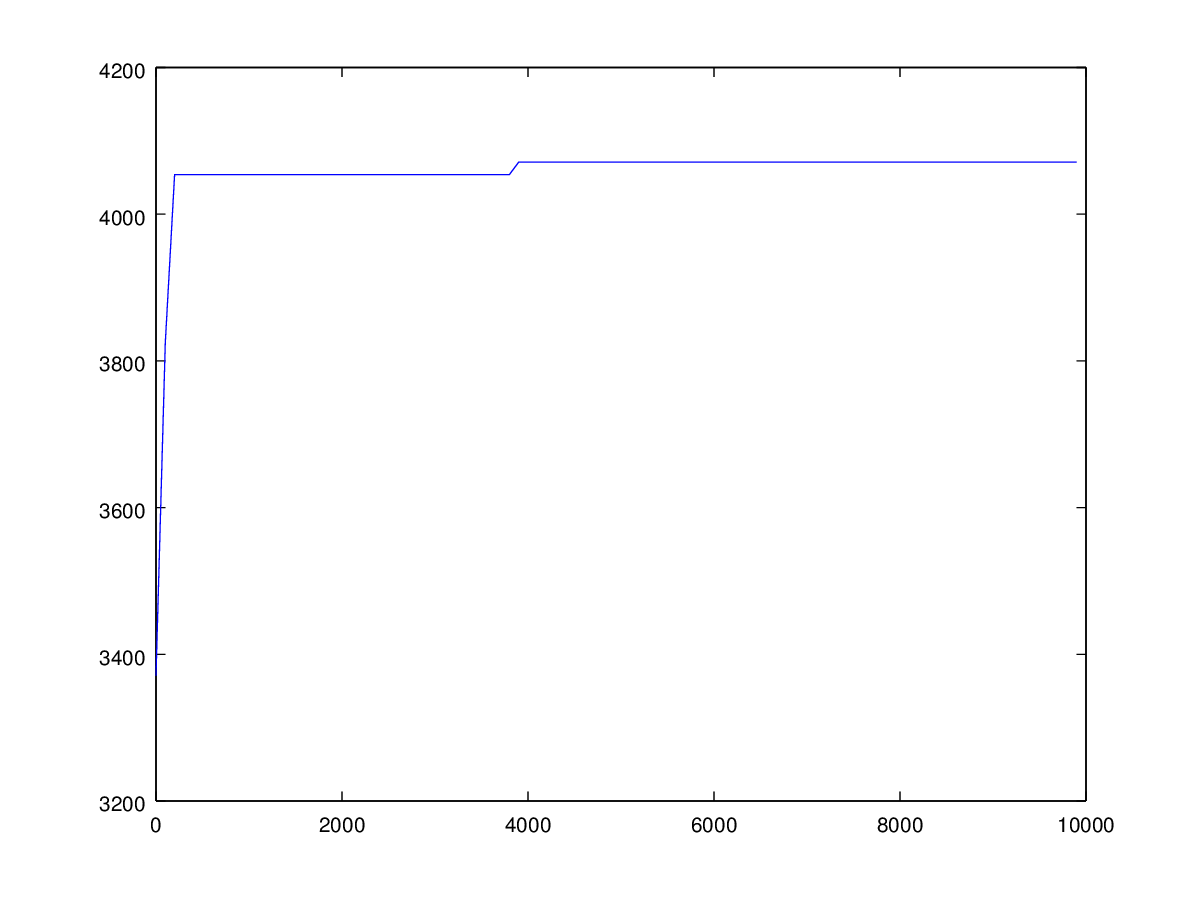
\includegraphics[width=0.5\textwidth]{images/graf_test_in.png}


\begin{IEEEeqnarray}{rCl}
Z&=&x_1 + x_2 + x_3 + x_4 + x_5 + x_6\IEEEnonumber\\
&&+\:a + b%
\end{IEEEeqnarray}

\begin{IEEEeqnarray}{Rl}
Z=&x_1 + x_2 + x_3 + x_4 + x_5 + x_6\IEEEnonumber\\
&+\:a + b%
\end{IEEEeqnarray}


\begin{IEEEeqnarray}{rCl}
A_1&=&7\IEEEyesnumber\IEEEyessubnumber\\
A_2&=&b+1\IEEEyessubnumber\\
\noalign{\noindent and\vspace{\jot}}A_3&=&d+2\IEEEyessubnumber%
\end{IEEEeqnarray}


\begin{IEEEeqnarray}[\setlength{\nulldelimiterspace}{0pt}]{rl,s}&x,&for $x \geq 0$\IEEEyesnumber\IEEEyessubnumber\\*
[-0.625\normalbaselineskip]
\smash{|x|=\left\{\IEEEstrut[3\jot][3\jot]\right.}&&
\nonumber\\*[-0.625\normalbaselineskip]
&-x,&for $x < 0$\IEEEyessubnumber
\end{IEEEeqnarray}


\begin{equation}
\label{eqn_example}
x = \sum\limits_{i=0}^{z} 2^{i}Q
\end{equation}
% ... as can be seen in (\ref{eqn_example}).


\setlength{\arraycolsep}{0.0em}
\begin{eqnarray}
Z&{}={}&x_1 + x_2 + x_3 + x_4 + x_5 + x_6\nonumber\\
&&+a + b\\
&&+{}a + b\\
&&{}+a + b\\
&&{+}\:a + b
\end{eqnarray}
\setlength{\arraycolsep}{5pt}


% Puntos a tocar en el informe:
% 	¿Qu\'e biblioteca fue utilizada?
% 	¿Qu\'e representaci\'on fue utilizada para las soluciones candidatas?
% 	¿Qu\'e estrategia fue utilizada para inicializar la poblaci\'on?
% 	¿Qu\'e operadores evolutivos fueron utilizados?
% 	¿C\'omo fue definida la funci\'on de fitness?
% 	Para el ejercicio 1:
% 		¿C\'ual fue la soluci\'on encontrada?
% 		¿Se encontr\'o m\'as de	una soluci\'on?
% 	Para el ejercicio 2:
% 		¿Qu\'e estrategia fue utilizada para el manejo de soluciones no factibles?



	\section{Conclusi\'on}
	Al final de este laboratorio hemos podido decicir aquella librer\'ia que se adapta mejor a nuestras necesidades y que nos gustar\'ia usar para resolver el proyecto final. Adem\'as, en el proceso de realizaci\'on de este primer pr\'actico, logramos interiorizarnos en aspectos pr\'acticos y la aplicaci\'on de algoritmos gen\'eticos y la s\'intesis de informes con Latex y otras herramientas.


% ------ Final ------

	\bibliographystyle{IEEEtran}
	\bibliography{informe.bib}{}

\end{document}